\section{Practical FEFF}

\begin{slide}{EXAFS Analysis strategy}

  \begin{center}
    \[ \chi(k) = \sum_j {\frac{{\Blue{N_j}} {\Red{f_j(k)}}
        e^{-2{\Blue{R_j}}/{\Red{\lambda(k)}}}
        e^{-2k^2{\Blue{\sigma_j^2}}}}{k{\Blue{R_j}}^2}
      {\sin[{2k{\Blue{R_j}} + {\Red{\delta_j(k)}}] }}} \]
  \end{center}

  We should be able to determine near-neighbor distance $R$ and
  coordination number $N$ and the structural disorder $\sigma^2$ if we know
  $\Red{f(k)}$, $\Red{\delta(k)}$, and $\Red{\lambda(k)}$.

  \onslide+<2->\vmm

  We can calculate these factors with a program called {\feff}.

  \onslide+<3->\vmm

  And then use these to determine $R$ and $N$ from experimental data.

   \vmm \hrule \vmm
   \onslide+<4->
  Topics to cover:
  \begin{itemize}
  \item How do we generate $\Red{f(k)}$, $\Red{\delta(k)}$,  and
    $\Red{\lambda(k)}$?
  \item What Correction Factors do we need to worry about?
  \item How do we fit experimental data?
  \item What tips and tricks can help fitting EXAFS data with {\feff}
    calculations?
  \end{itemize}

\end{slide}

\begin{slide}{{\feff} Overview (What does {\feff} do?)}

  {\feff} calculates $\Red{f(k)}$ and $\Red{\delta(k)}$
  for all  {\RedEmph{Scattering Paths}}  in a cluster of atoms:

  How does it do this?

  \begin{enumerate}
    \onslide+<2->\item  build atomic potentials (how will electrons
    interact with an atom).
    \onslide+<3->{To  simplify the calculations,

      \begin{center}
        \begin{tabular}{ll}
          \begin{minipage}{80mm}
            Use the {\BlueEmph{Cup-Cake Tin Approximation}}:
            atomic potentials up to a uniform Fermi level:
            No Chemical Bonding!

            {\onslide+<3->\hspace{4mm}(aka  Muffin-Tin Approximation)}
          \end{minipage}
          &
          \begin{minipage}{25mm}
            {\onslide+<2-> 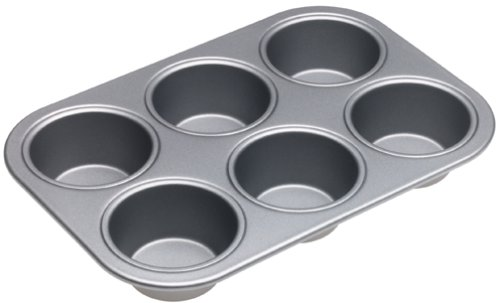
\includegraphics[width=20mm]{figs/Images/muffintin2}}
          \end{minipage}
        \\
      \end{tabular}
    \end{center}
  }

  \onslide+<4->\item determine important scattering paths.

    \begin{itemize}
    \item Build paths from a selected {\BlueEmph{central atom}} in a cluster of atoms.
    \item Decide which paths are the same atom types and path length
      (``degenerate'').
    \item Decide which paths are unimportant for XAFS.
    \end{itemize}

  \onslide+<5->\item move photo-electron along path to determine
    $\Red{f}$ and $\Red{\delta}$ as a function of $k$:

    \begin{center}
      propagate $\Rightarrow$ scatter $\Rightarrow$ propagate $\Rightarrow$ \ldots.
    \end{center}

  \end{enumerate}

\end{slide}

\begin{slide}{{\feff}: what's so hard about that?}

  {\feff} includes sophisticated techniques  to
  calculate \feffc{f(k)} and \feffc{\delta(k)}:

    \vmm \vmm

    \begin{description}[POLARIZA]
    \item[\RedEmph{Curved Wave Effects}] the photo-electron goes out as
      spherical wave and scatters from atoms with finite size.

    \item[\RedEmph{Extrinsic Losses}] {\feffc{\lambda(k)}}: self-energy and
      core-hole lifetime.

    \item[\RedEmph{Intrinsic Losses}] {\feffc{S_0^2}}: the absorbing atom
      relaxes to the presence of the core hole.

    \item[\RedEmph{Multiple Scattering}]  the photo-electron can scatter
      multiple times. Most important at low $k$ and for \BlueEmph{linear paths}.

    \item[\RedEmph{Polarization Effects}] synchrotron beams are highly
      polarized, which needs to be taken into account.  This is simple for
      $K$-edges ($s\rightarrow p$ is dipole), but more complicated for $L$
      and $M$ (and higher) shells.

    \end{description}

\end{slide}


\begin{slide}{ Practical {\feff} }

{\RedEmph{Good News}}: you don't have to worry about most of this!

\vmm
\pause
The normal scheme for using {\feff} for EXAFS data analysis  is:

\begin{enumerate}
\item Start with a structure close to the {\BlueEmph{local}} atomic structure
  of your sample, and generate x,y,z coordinates for the atoms.
  \begin{itemize}
    \item simple crystal structure?   use {\RedEmph{\Program{atoms}}} input
      format or look up at
      {\webpage{http://cars9.uchicago.edu/~newville/adb/search.html}}
    \item Protein Data Bank?          use {\RedEmph{\Program{crystalff}}}
    \item Something Else?   use atomic coordinates, modify
      existing input file.
  \end{itemize}
  \pause
\item Run {\feff}.  This creates a {\feffndat} files for each
  path in your structure.
  \pause
\item Use these  Path Files in to model measured XAFS in an analysis
  program.
\end{enumerate}

\vmm \pause
{\artemis} makes this even easier: it runs and manages {\feff} for you.

% \vmm \pause
% You may need to use a few structures to find appropriate paths for your system.

\vmm \pause

\begin{cenpage}{80mm}
  Having good starting structures can be important, but you do not need the
  exact structure to use {\feff}.
\end{cenpage}

\end{slide}

\subsection{Anatomy of {\file{feff.inp}}}
\begin{frame}[fragile] \frametitle{Anatomy of {\file{feff.inp}}}

{\feff} is a very old program that runs from an input file -- it
{\bf{must}} be called {\file{feff.inp}}.  No Kidding!

\onslide<2->

\begin{tabular}{lr}
  \begin{CodeBlock}{51mm}{\file{feff.inp} file:}
{\Blue{TITLE    FeO, rock salt structure}}

{\Blue{HOLE     1   1.0}}   {\Red{\# K Edge, S02}}
{\Blue{CONTROL  1 1 1 1}}   {\Red{\# which parts of code to run}}
{\Blue{PRINT    1 0 0 3}}   {\Red{\# which output files to write}}

{\Blue{POTENTIALS }}        {\Red{\# list of Atomic Potentials}}
 * potential   z  label
       0      26   Fe    {\Red{\# Absorbing Atom  Potential=0}}
       1       8   O     {\Red{\# 1 Potential for each Z}}
       2      26   Fe

{\Blue{ATOMS}}  {\Red{\# list of Atomic X, Y, Z, Potential }}
  0.00000     0.00000     0.00000    0   Fe
  0.00000     0.00000    -2.13870    1   O
 -2.13870     0.00000     0.00000    1   O
  0.00000    -2.13870     0.00000    1   O
  0.00000     0.00000     2.13870    1   O
  2.13870     0.00000     0.00000    1   O
  0.00000     2.13870     0.00000    1   O
  0.00000     2.13870     2.13870    2   Fe
  0.00000    -2.13870    -2.13870    2   Fe
 -2.13870     2.13870     0.00000    2   Fe
  2.13870    -2.13870     0.00000    2   Fe
  0.00000    -2.13870     2.13870    2   Fe
\end{CodeBlock} &
\begin{minipage}{62mm}
\onslide<3->

{\file{feff.inp}} includes:
\begin{enumerate}
  \onslide<4->\item A list of unique Atomic Potentials:
  \begin{itemize}
  \item Pot 0 = Absorbing Atom
  \item 1 Potential per atomic species (Z)
  \end{itemize}

  \onslide<5->\item List of atomic coordinates:

  {\hmm} $x$, $y$, $z$, $Pot$

  for the cluster of atoms (in {\AA}).

  \vmm
  The cluster does not need to be a crystal structure!

  \vmm
  The absorbing atom does not have to be at 0,0,0

\end{enumerate}
\end{minipage}\\
\end{tabular}
\end{frame}


\begin{slide}{Input Parameters for {\file{feff.inp}}}

  {\feff} has many  inputs, but only a few of them are really
  important for EXAFS Analysis (some are {\Red{\texttt{required}}}, some {\Blue{\texttt{optional}}}):


  \begin{description}[POTENTIALSXX]
  \item[{\Red{\texttt{HOLE}}}]   which orbital absorbs the x-ray (1 = $K$, 4
    = $L_{\rm III}$ )

  \item[{\Red{\texttt{POTENTIALS}}}]   list of atomic potentials (0 = absorbing atom)

  \item[{\Red{\texttt{ATOMS}}}]   list of atomic $x$, $y$, $z$, Potential

  \item[{\Red{\texttt{CONTROL}}}]   which ``Modules'' to run.  Use  ``1 1 1 1''.

  \item[{\Red{\texttt{PRINT}}}]   which ``Outputs'' to write. Use  ``1 0 0 0''.


    \pause
  \item[{\Blue{\texttt{RMAX}}}]   how far out (in {\AA}) to consider the
    cluster of atoms.

  \item[{\Blue{\texttt{POLARIZATION}}}]   polarization vector of incident
    x-ray (in same coordinate system as atomic coordinates)

  \item[{\Blue{\texttt{EXCHANGE}}}]   which model to use for the exchange energy.
    Use the default (Hedin-Lundqvist model) unless you know why.

  \end{description}

\end{slide}


\subsection{{\scshape{atoms}} and {\file{atoms.inp}}}
\begin{frame}[fragile] \frametitle{{\scshape{atoms}} and {\file{atoms.inp}}}

One convenient way to make {\file{feff.inp}} is with the {\atoms} program
which converts  Crystal Structure to Atomic Cluster:

\begin{tabular}{lr}
  \begin{CodeBlock}{48mm}{\file{atoms.inp} file:}
{\Blue{TITLE    FeO, rock salt structure}}

{\Blue{space f m 3 m}}   {\Red{\# Space Group}}

{\Blue{a  = 4.2774}}     {\Red{\# Lattice Constant}}
{\Blue{rmax = 6.00}}     {\Red{\# Cluster Size}}
{\Blue{core = Fe1}}      {\Red{\# Central Atom}}

{\Blue{atom}}    {\Red{\# List of Cell Parameters}}
Fe    0.0000   0.0000   0.0000  Fe1
O     0.5000   0.5000   0.5000  O1
------
\end{CodeBlock} &
\begin{minipage}{58mm}
\onslide+<2->

Using {\atoms} is convenient, but not necessary!

\vmm \vmm
{\atoms} does not allow ``doping'', or fractional substitution -- you must
edit the {\file{feff.inp}} file for that!!

\end{minipage}\\
\end{tabular}

\onslide+<3->
\begin{postitbox}{84mm}
  The cluster used by {\feff} does not need to be a crystal!
\end{postitbox}

\vmm
Atomic clusters may also come from:

\vmm
Protein Data Bank, CIF Format data,
Density Functional Theory Calculations, \ldots.

\end{frame}


\subsection{ {\file{feffNNNN.dat}}: {\feff}'s output}
\begin{frame}[fragile] \frametitle{ {\file{feffNNNN.dat}}: {\feff}'s output}

  {\feff} writes out a separate file for each Scattering Path:

  {\file{feff0001.dat}}, {\file{feff0002.dat}}, \ldots

  indexed by path length.


  \begin{tabular}{ll}
  \begin{CodeBlock}{74mm}{\file{feff.dat} file:}
FeO, rock salt structure                                   Feff XX 6.10
Abs   Z=26 Rmt= 1.197 Rnm= 1.402 K shell
Pot 1 Z= 8 Rmt= 0.937 Rnm= 1.103
Pot 2 Z=26 Rmt= 1.203 Rnm= 1.418
Gam\_ch=1.325E+00 H-L exch
Mu=-4.210E+00 kf=2.067E+00 Vint=-2.048E+01 Rs\_int= 1.755
Path    1      icalc       2
-----------------------------------------------------------------------
{\Red{ 2   1.000   2.1387    2.4356   -4.21002 nleg, deg, reff, rnrmav(bohr), edge}}
{\Blue{       x         y         z   pot at}}
    0.0000    0.0000    0.0000  0  26 Fe       absorbing atom
    0.0000    2.1387    0.0000  1   8 O
{\Red{ k   real[2*phc]   mag[feff]  phase[feff] red factor   lambda    real[p]}}
   0.000  2.9505E+00  0.0000E+00 -3.0508E+00  0.1009E+01  2.3773E+01  2.0669E+00
   0.200  2.9485E+00  9.9421E-02 -3.8738E+00  0.1009E+01  2.3876E+01  2.0762E+00
   0.400  2.9424E+00  1.9477E-01 -4.6322E+00  0.1009E+01  2.4141E+01  2.1037E+00
   0.600  2.9320E+00  2.8278E-01 -5.3276E+00  0.1010E+01  2.4444E+01  2.1488E+00
   0.800  2.9172E+00  3.6142E-01 -5.9621E+00  0.1011E+01  2.4599E+01  2.2105E+00
   1.000  2.8976E+00  4.2991E-01 -6.5379E+00  0.1012E+01  2.4410E+01  2.2878E+00
   1.200  2.8723E+00  4.8834E-01 -7.0570E+00  0.1014E+01  2.3748E+01  2.3798E+00
\end{CodeBlock}
&
  \begin{minipage}{35mm}
    This file contains:
    \begin{enumerate}
    \item Path geometry
    \item Data for $f(k)$,  $\delta(k)$, and  $\lambda(k)$.
    \end{enumerate}
    \vmm \onslide+<2->
    You {\RedEmph{never}} have to read this file -- the analysis program
    will do that.

    \vmm You may have to move and/or rename the file.

  \end{minipage}\\
  \end{tabular}

\onslide+<3->
\vmm Analysis programs will use these files (or Phases \& Amplitudes from
them) to model EXAFS as a {{Sum Over Paths}}.

\end{frame}

\begin{slide}{ {\feff}: What {\em{Should}} you worry about?}

  Using {\feff} in a real analysis, we'll be {\BlueEmph{refining}}
  bond lengths and coordination numbers.  For this to work, here are some
  ``rules of thumb'':

  \begin{cenpage}{90mm}

\begin{enumerate}
  \pause \item  refining atomic distances by more than $0.1\rm\,\AA$
  probably means the calculation should be re-run -- the overlap of atomic
  potentials may not be accurate.


  \pause \item  refining energy origins $E_0$ by more than $10\rm\,eV$ may
  mean the calculation -- or the selection of $E_0$ in the data reduction
  -- needs to be re-examined.

  \pause \item  {\feff} can set $S_0^2$ and make a simple attempt at
  $\sigma^2$ values.  This confuses the analysis, so don't use them.

  \pause \item  You probably do need to adjust an $S_0^2$ for a particular
  set of data (central atom, beamline energy resolution, etc)
  \end{enumerate}
  \end{cenpage}

\end{slide}

\section{Correction Factors}

%% Slide
\begin{slide}{$S_0^2$:  Amplitude Reduction Term}

  An important correction for EXAFS is the {\Red{Amplitude Reduction
      Term}}, due to the relaxation of the {\BlueEmph{other electrons in
      the absorbing atom}} to the hole in the core level:

   \vmm
   \[
   S_0^2 =  {  |{\langle \Phi^{N-1}_f |\Phi^{N-1}_0 \rangle}|^2}
   \]

   \vmm

   ${| \Phi^{N-1}_0 \rangle }$ = $(N-1)$ electrons in unexcited atom.

   ${\langle \Phi^{N-1}_f|}$   = $(N-1)$ electrons, relaxed by core-hole.

   \vmm

   \onslide+<2->
   ${S_0^2}$ is usually taken as a constant:

   \begin{postitbox}{25mm}
     $ 0.7 < S_0^2 < 1.0 $
   \end{postitbox}

  and is used as a Fitting Parameter that multiplies {$\chi$}:

  \vmm  \onslide+<3->

  \begin{center}
    {\Red{ ${S_0^2}$ is Completely Correlated with $N$      (!!!)}}
  \end{center}

  \vmm \onslide+<3->

   \begin{postitbox}{75mm}
     This make EXAFS amplitudes (and therefore {\Blue{$N$}}) less precise
     than EXAFS phases (and therefore {\Blue{$R$}}).
  \end{postitbox}


\vfill
\end{slide}


%% Slide
\begin{slide}{$\lambda$: Photo-Electron Mean Free Path}

  \vmm
    The photo-electrons that scatter to give EXAFS can also scatter
    {\RedEmph{inelastically }} (lose energy).

    \vmm\pause
    In addition, the {\RedEmph{core hole}} (empty electronic level)
    will eventually re-fill.

    \vmm\onslide+<3->

    These two effects combine to give a {\BlueEmph{mean
        free path}},  ${\lambda(k)}$:

    \vmm
   \begin{postitbox}{66mm}
    How far can the  photo-electron go and still make it back to the
    excited absorbing atom?
   \end{postitbox}

    \vmm\onslide+<4->
    To model this, the photo-electron wavefunction becomes:

    \[ \displaystyle{
        \psi(k,r)  =  {\frac{e^{ikr}}{kr}}
        \Rightarrow   {\frac{e^{ikr}e^{-r/\lambda(k)}}{kr}}
        }
    \]

    which gives the

    \[        e^{-2{\Blue{R_j}}/{\Red{\lambda(k)}}} \]

    term in the EXAFS equation.



\vfill
\end{slide}

%% Slide
 \begin{slide}{${\lambda(k)}$: The Photo-Electron Mean-Free Path}

   \begin{center}
       \scalebox{1}{\wgraph{70mm}{theory/scatt_lam}}
     \end{center}

     \vmm

     \begin{itemize}
       \item ${\rm 5 \AA < \lambda < 50\,\AA}$ for the EXAFS ${k}$-range.

       \item The ${\lambda}$ and ${R^{-2}}$ terms in the EXAFS equation
         make EXAFS a  {\RedEmph{local probe}}.

       \item  XANES ( $k<3\rm\,\AA^{-1}$ ) is more sensitive to larger
         distances.
       \end{itemize}
\vfill
\end{slide}

%% Slide
\begin{slide}{${p(k)}$: the complex momentum of the photo-electron }

  With

    \[ \displaystyle{{
        \psi(k,r)  =  {\frac{e^{ikr}}{kr}}
        \Rightarrow   {\frac{e^{ikr}e^{-r/\lambda(k)}}{kr}}
        \onslide+<2->
        \Rightarrow {\frac{e^{ipr}}{pr}} }}
    \]

    we can use a {\RedEmph{complex wavenumber}} of the photo-electron:

    \[{p(k) = k + i / \lambda(k) } \]

    \onslide+<3->
    By itself, this is not terribly important, but I'll use $p$ in the next
    few slides.

    \vfill
\end{slide}


% \begin{slide}{XAFS Analysis with {\feff} }

%   Finally, the XAFS Equation used with {\feff}:

%   \[
%   \chi(k) = \sum_j {{{\Blue{N_j}} S_0^2 {\Red{f_j(k)}}  e^{-2R_j/\lambda(k)}
%       e^{-2k^2{\Blue{\sigma_j^2}}}}\over{k{\Blue{R_j}}^2}}
%   {\sin[{2k{\Blue{R_j}} + {\Red{\delta_j(k)}}} ]}
%    \]

%    \begin{itemize}
%    \onslide+<2->\item  The sum is over  {\RedEmph{Scattering Paths}} of the
%    photo-electron.   Both:

%    \begin{description}[MultipleXXScatteringX]

%    \item[Single Scattering] {\tiny{ absorbing atom $\Rightarrow$ neighbor atom
%      $\Rightarrow$ absorbing atom}}


%    \item[Multiple Scattering] {\tiny{absorbing atom $\Rightarrow$ neighbor
%      atom  $\Rightarrow$ neighbor atom $\Rightarrow$ \ldots  $\Rightarrow$
%      absorbing atom}}

%    \end{description}

%    \onslide+<3->\item $\Red{f(k)}$ and $\Red{\delta(k)}$ are
%    {{photo-electron scattering amplitude and phases}}:

%    \begin{itemize}
%    \item Energy ($k$) dependent.
%    \item $Z$ dependent -- $Z$ of the scattering atoms(s).
%    \item non-trivial: must be calculated (or extracted from measured spectra).

%    \end{itemize}
%  \end{itemize}

%    \vmm \hrule \vmm

%    \onslide+<4->

%    Knowing  $\Red{f(k)}$ and $\Red{\delta(k)}$, we can determine structural
%    information:
%      \begin{itemize}
%      \item ${\Blue{R}}$ --  near neighbor distance.
%      \item ${\Blue{N}}$ -- coordination number.
%      \item ${\Blue{\sigma^2}}$ -- mean-square  disorder in ${\Blue{R}}$.
%      \end{itemize}
%    \vmm

% \end{slide}


% \begin{slide}{End of Feff practice }
%   \vfill
%   \begin{center}
%      \begin{postitbox}{37mm}
%        \Huge{Questions?}
%    \end{postitbox}
%   \end{center}
%   \vfill
%  \end{slide}


